A partir dos dados analisados, foi possível modelar o problema utilizando o software de simulação Arena. A Figura \ref*{fig: ACD} mostra o Diagrama de Ciclo de Atividades (ACD) que auxiliou na modelagem computacional do problema. A Figura \ref*{fig: modelo-arena} apresenta o modelo implementado no Arena. O módulo \textit{Create} nomeado "Chegada"\;recebe uma distribuição de tempo entre chegadas de acordo com os valores modelados na Seção \ref*{section: fit-arrivals}. O módulo \textit{Process} nomeado "Atendimento"\;realiza as ações de \textit{seize}, \textit{delay} e \textit{release} com tempo conforme distribuição exponencial com média 299,1 segundos. São utilizados módulos \textit{Assign} para criar atributos de instante de chegada ("call\_started"), tipo de ligação ("call\_type"), instante de atendimento da chamada ("call\_answered") e instante de fim do atendimento ("call\_ended"). Estes atributos são escritos pelo Arena em um arquivo em formato CSV para posterior análise dos dados.

\begin{figure}[H]
    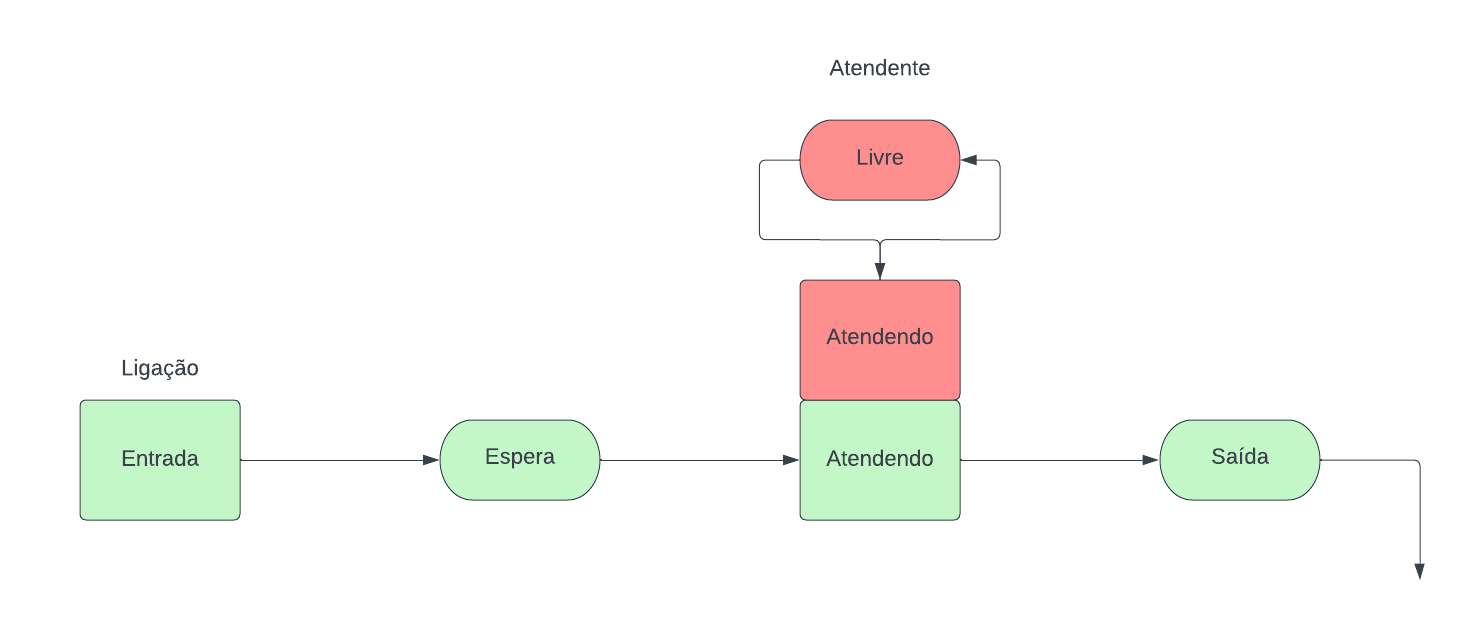
\includegraphics[scale=0.3]{simulacao/acd_vcbc.png}
    \caption{Diagrama de Ciclo de Atividades de uma central de atendimentos}
    \label{fig: ACD}
\end{figure}

\begin{figure}[H]
    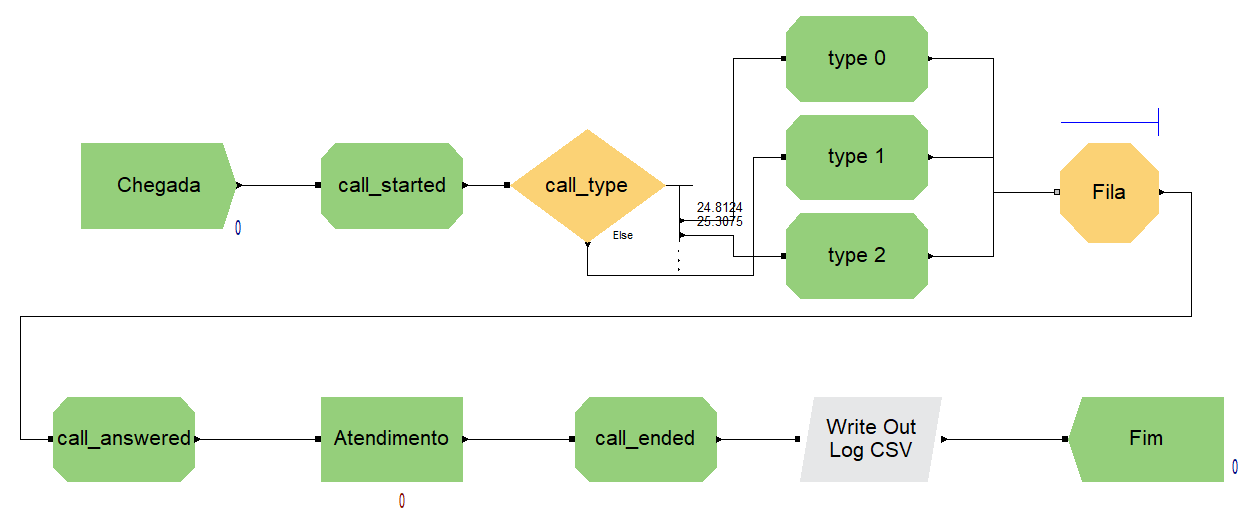
\includegraphics[scale=0.6]{simulacao/modelo-arena.png}
    \caption{Modelo de simulação implementado no Arena}
    \label{fig: modelo-arena}
\end{figure}

A estrutura do arquivo de saída do Arena pode ser vista na Figura \ref*{fig: csv-arena}, após tratamento em Python. Todos os intervalos e instantes registrados estão em segundos.

\begin{figure}[H]
    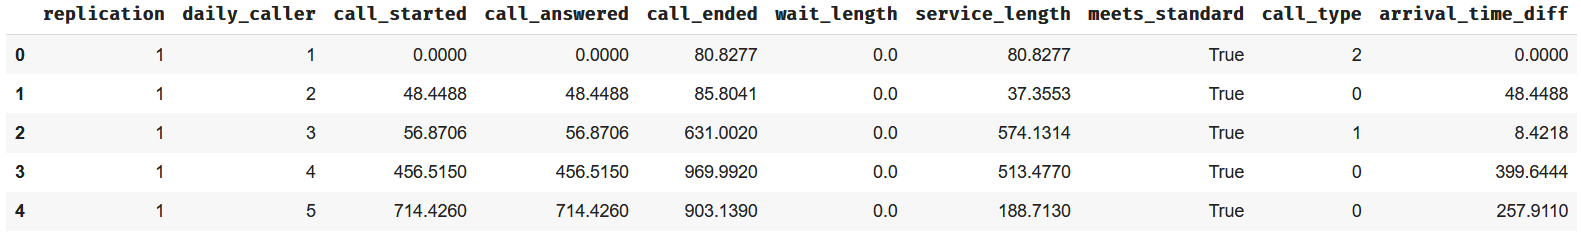
\includegraphics[scale=0.45]{simulacao/csv-arena.png}
    \caption{Primeiras 5 linhas de uma amostra gerada pela simulação no Arena}
    \label{fig: csv-arena}
\end{figure}

\subsection{Validação do modelo}
Para validação do modelo foram realizados testes de hipóteses utilizando o teste de Kolmogorov-Smirnov de 2 amostras para determinar se os valores simulados estão de acordo com os valores históricos. A Tabela \ref*{fig: teste-modelo-historico} apresenta os valores $p$ calculados para cada mês, comparando as amostras dos meses simulados aos valores registrados, assim como o número de replicações aplicado na criação de cada amostra da simulação. Há a rejeição da hipótese nula em três tempos de serviço modelados (valor $p < 0,05$), nos meses de fevereiro, outubro e dezembro.

\begin{table}[H]
    \centering
    \begin{tabular}{|r|r|r|r|r|}
    \hline
     & wait\_length & service\_length & arrival\_time\_diff & Replicações \\ \hline
    Janeiro & 1 & 0,6 & 0,6339 & 21 \\ \hline
    Fevereiro & 1 & \circletext{0,0317} & 0,3055 & 20 \\ \hline
    Março & 1 & 0,6993 & 0,8848 & 23 \\ \hline
    Abril & 0,9898 & 0,09 & 0,1995 & 22 \\ \hline
    Maio & 1 & 0,0869 & 0,5306 & 21 \\ \hline
    Junho & 1 & 0,096 & 0,8442 & 22 \\ \hline
    Julho & 0,9983 & 0,235 & 0,7632 & 22 \\ \hline
    Agosto & 0,4519 & 0,1326 & 0,6323 & 22 \\ \hline
    Setembro & 0,9999 & 0,2445 & 0,8099 & 22 \\ \hline
    Outubro & 0,8217 & \circletext{0,0218} & 0,4198 & 21 \\ \hline
    Novembro & 0,7347 & 0,381 & 0,4229 & 22 \\ \hline
    Dezembro & 0,3517 & \circletext{0,0334} & 0,386 & 23 \\ \hline
    \end{tabular}
    \caption{Valores $p$ dos testes de validação dos tempos do modelo}
    \label{fig: teste-modelo-historico}
\end{table}
    
    
Foi realizado um redimensionamento do número de replicações para tentar compreender a rejeição dos valores obtidos para tempos de serviço. A Tabela \ref*{fig: intervalo-confianca} apresenta, para o mês de dezembro, os intervalos de confiança dos tempos obtidos com 5\% de significância. Para aumentar a precisão dos tempos de serviço, que apresentam maior variância e foram rejeitados no teste de hipótese, foi dimensionado o número de amostras necessárias ($n^*$) para uma precisão desejada ($h^*$) de 3,5 segundos, conforme Tabela \ref*{fig: dimensionamento-corridas}. Como cada replicação deste mês tem em média 270 chamadas, consideramos o valor de 100 replicações para atingir o número de amostras calculado.

\begin{table}[H]
    \begin{tabular}{|l|r|r|r|r|r|r|r|r|r|}
    \hline
    Tempo & \multicolumn{1}{l|}{n} & \multicolumn{1}{l|}{Confiança} & \multicolumn{1}{l|}{$\alpha$} & \multicolumn{1}{l|}{$t$ stat} & \multicolumn{1}{l|}{Desv. Pad.} & \multicolumn{1}{l|}{h} & \multicolumn{1}{l|}{LI} & \multicolumn{1}{l|}{$\mu$} & \multicolumn{1}{l|}{LS} \\ \hline
    Espera & 6213 & 95,00\% & 5,00\% & 1,9603 & 116,0300 & 2,8857 & 39,8890 & 42,7747 & 45,6604 \\ \hline
    Serviço & 6213 & 95,00\% & 5,00\% & 1,9603 & 286,2428 & 7,1190 & 279,8161 & 286,9351 & 294,0540 \\ \hline
    Entre chegadas & 6213 & 95,00\% & 5,00\% & 1,9603 & 134,3537 & 3,3414 & 128,8882 & 132,2297 & 135,5711 \\ \hline
    \end{tabular}
    \caption{Intervalos de confiança das médias dos tempos simulados para o mês de dezembro}
    \label{fig: intervalo-confianca}
\end{table}

\begin{table}[H]
    \centering
    \begin{tabular}{|l|l|l|l|}
    \hline
    n* & n & h & h* \\ \hline
    \multicolumn{1}{|r|}{25703,864} & \multicolumn{1}{r|}{6213} & \multicolumn{1}{r|}{7,1190} & \multicolumn{1}{r|}{3,5} \\ \hline
    \end{tabular}
    \caption{Dimensionamento do número de amostras necessário para maior precisão na validação do modelo}
    \label{fig: dimensionamento-corridas}
\end{table}
    
Executando a validação do modelo com 100 replicações para cada mês, temos na Tabela \ref*{fig: teste-modelo-historico-100} os valores $p$ da comparação das amostras dos meses simulados aos valores históricos, além do percentual médio de falhas em cada mês da simulação, definido como a porcentagem de ligações que levaram mais de 1 minuto para serem atendidas. Neste caso, nenhum $p$ valor ficou abaixo do nível de significância estipulado de 5\%, comprovando que o modelo é bom o suficiente para representar o comportamento dos dados reais em cada um dos meses.

\begin{table}[H]
    \centering
    \begin{tabular}{|l|r|r|r|r|r|}
    \hline
     & \multicolumn{1}{l|}{wait\_length} & \multicolumn{1}{l|}{service\_length} & \multicolumn{1}{l|}{arrival\_time\_diff} & \multicolumn{1}{l|}{Replicações} & \multicolumn{1}{l|}{\% médio de falhas} \\ \hline
    Janeiro & 1 & 0,3175 & 0,311 & 100 & 2,33\% \\ \hline
    Fevereiro & 1 & 0,3135 & 0,0561 & 100 & 2,67\% \\ \hline
    Março & 1 & 0,5948 & 0,685 & 100 & 3,11\% \\ \hline
    Abril & 0,8847 & 0,1727 & 0,0609 & 100 & 3,67\% \\ \hline
    Maio & 1 & 0,561 & 0,3087 & 100 & 4,14\% \\ \hline
    Junho & 1 & 0,4937 & 0,7136 & 100 & 4,73\% \\ \hline
    Julho & 1 & 0,7783 & 0,5795 & 100 & 5,94\% \\ \hline
    Agosto & 0,8023 & 0,6972 & 0,548 & 100 & 7,34\% \\ \hline
    Setembro & 0,971 & 0,8679 & 0,5704 & 100 & 10,27\% \\ \hline
    Outubro & 0,9968 & 0,2854 & 0,8972 & 100 & 11,93\% \\ \hline
    Novembro & 0,148 & 0,7403 & 0,0843 & 100 & 14,59\% \\ \hline
    Dezembro & 0,0719 & 0,6286 & 0,2675 & 100 & 18,17\% \\ \hline
    \end{tabular}
    \caption{Valores $p$ dos testes de validação dos tempos do modelo realizando 100 replicações}
    \label{fig: teste-modelo-historico-100}
\end{table}
    
\subsection{Teste de capacidade da central de atendimentos}
Para avaliar o volume máximo de chamadas que podem ser atendidas sem violar a meta de 90\% das chamadas atendidas em até 1 minuto, isto é, trabalhando com menos de 10\% de falhas, podemos utilizar o modelo de simulação com distribuição dos intervalos entre chegadas próximos do valor modelado para o mês de setembro, no qual o sistema deixa de cumprir a meta, e cuja média do tempo entre chegadas é de 156,4994 segundos. A Tabela \ref{tab: stress-test} apresenta os testes realizados para avaliação da capacidade, executando 100 replicações para cada tempo entre chegadas testado. O volume máximo que pode ser tratado por dia é, em média, 229 chamadas.

\begin{table}[H]
    \centering
    \begin{tabular}{|r|r|r|}
    \hline
    \multicolumn{1}{|l|}{Tempo médio entre chegadas (s)} & \multicolumn{1}{l|}{Quantidade média de chegadas} & \multicolumn{1}{l|}{\% falha} \\ \hline
    160 & 225,14 & 9,64\% \\ \hline
    159 & 226,6 & 9,67\% \\ \hline
    158 & 228,15 & 9,88\% \\ \hline
    157 & 229,59 & 10,11\% \\ \hline
    \end{tabular}
    \caption{Resultados do teste de capacidade da central de atendimento}
    \label{tab: stress-test}
 \end{table}